% IF YOU ARE USING OVERLEAF, MAKE SURE TO SET THE COMPILER TO XeLatex (Menu in the top left > Settings > Compiler).

% Gemini theme
% See: https://rev.cs.uchicago.edu/k4rtik/gemini-uccs
% A fork of https://github.com/anishathalye/gemini

\documentclass[final]{beamer}

% ====================
% Packages
% ====================

\usepackage[T1]{fontenc}
\usepackage{lmodern}
\usepackage[size=custom,width=120,height=72,scale=1.0]{beamerposter}
\usetheme{gemini}
% \usecolortheme{uchicago}
\usecolortheme{stanford}
\usepackage{graphicx}
\usepackage{booktabs}
\usepackage{tikz}
\usepackage{pgfplots}
\pgfplotsset{compat=1.17}

% ====================
% Lengths
% ====================

% If you have N columns, choose \sepwidth and \colwidth such that
% (N+1)*\sepwidth + N*\colwidth = \paperwidth
\newlength{\sepwidth}
\newlength{\colwidth}
\setlength{\sepwidth}{0.025\paperwidth}
\setlength{\colwidth}{0.3\paperwidth}

\newcommand{\separatorcolumn}{\begin{column}{\sepwidth}\end{column}}


\title{Direct Preference Optimization: From Paraphrase Detection to Shakespearean Sonnet Generation}


\author{Florencio Paucar}

\institute[shortinst]{Department of Computer Science, Stanford University}

% ====================
% Footer (optional)
% ====================

\footercontent{
  \href{mailto:fpaucar@stanford.edu}{fpaucar@stanford.edu} \hfill
  Stanford CS224N Default Project \hfill
  }
% (can be left out to remove footer)

% ====================
% Logo (optional)
% ====================

% use this to include logos on the left and/or right side of the header:
% \logoright{\includegraphics[height=7cm]{logos/cs-logo-maroon.png}}
% \logoleft{\includegraphics[height=7cm]{logos/cs-logo-maroon.png}}

% ====================
% Body
% ====================

\begin{document}

% This adds the Logos on the top left and top right
\addtobeamertemplate{headline}{}
{
    \begin{tikzpicture}[remember picture,overlay]
    %   \node [anchor=north west, inner sep=3cm] at ([xshift=0.0cm,yshift=1.0cm]current page.north west)
    %   {\includegraphics[height=5.0cm]{stanford_logos/Stanford-CS.png}}; % uc-logo-white.eps
      \node [anchor=north east, inner sep=3cm] at ([xshift=0.0cm,yshift=2.5cm]current page.north east)
      {\includegraphics[height=7.0cm]{stanford_logos/Block_S_2_color.png}};
    \end{tikzpicture}
}

\begin{frame}[t]
\begin{columns}[t]
\separatorcolumn

\begin{column}{\colwidth}

  \begin{block}{Problem}

    Aligning language models with human preferences has become a central challenge in NLP. While \textbf{Reinforcement Learning from Human Feedback (RLHF)} achieves strong results, its complexity, requiring simultaneous management of multiple models and costly online sampling, motivates simpler alternatives.
    
    \textbf{Direct Preference Optimization (DPO)} addresses this by reformulating alignment as a classification problem, eliminating the need for an explicit reward model. However, DPO's effectiveness has been evaluated almost exclusively on open-ended generation tasks.
    
    \begin{figure}
        \centering
        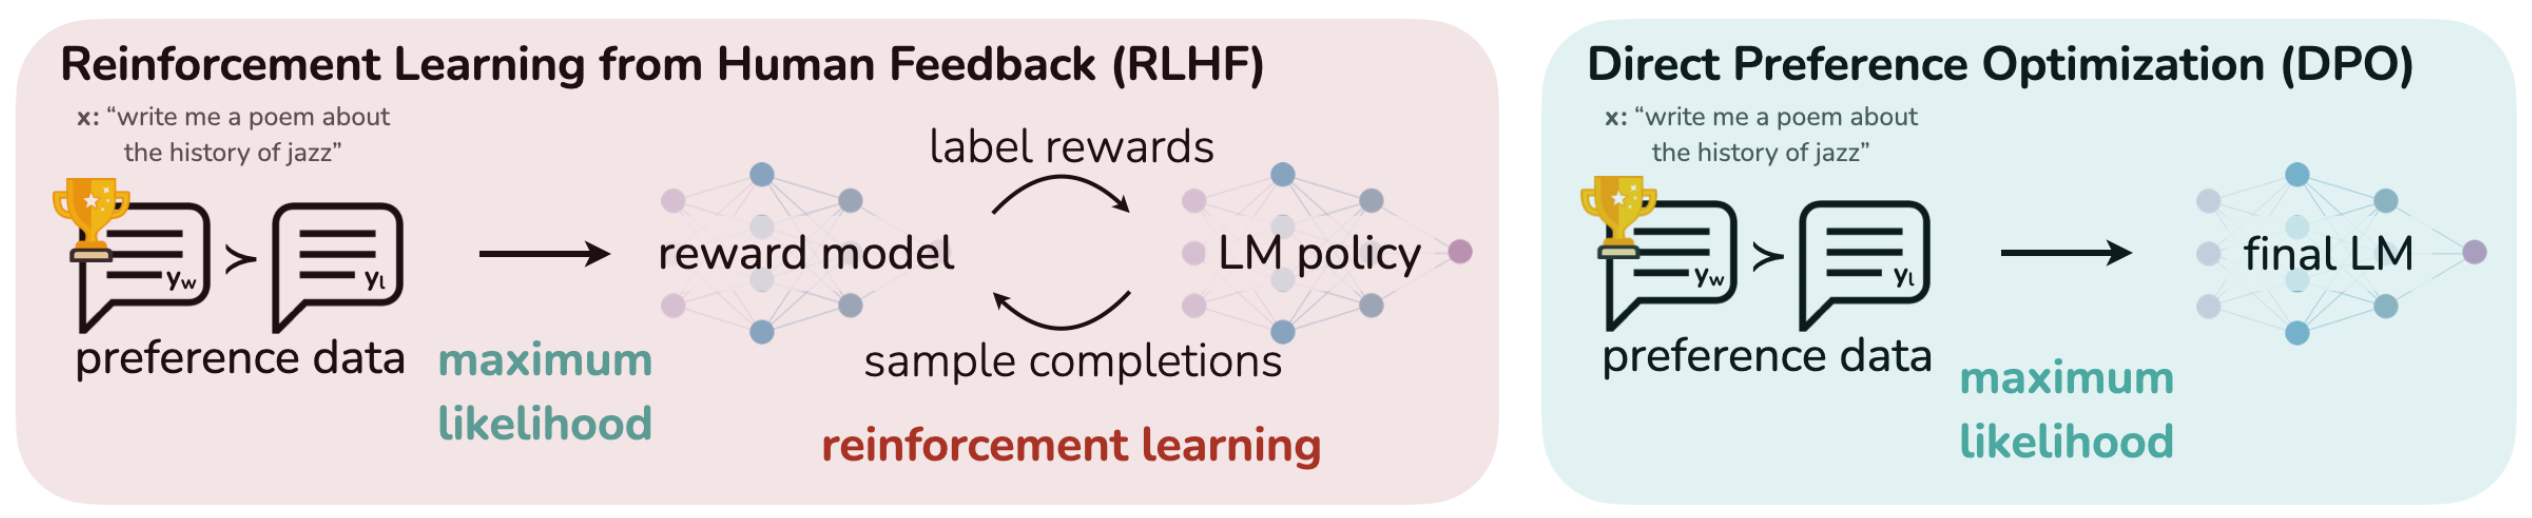
\includegraphics[width=1\linewidth]{images/original-dpo-image.png}
        \caption{DPO optimizes for human preferences while avoiding reinforcement learning~\cite{rafailov2024directpreferenceoptimizationlanguage}.}
        \label{fig:original-dpo}
    \end{figure}

    \textbf{Goal:} This work presents a comprehensive empirical evaluation of DPO applied to two underexplored tasks: paraphrase detection and Shakespearean sonnet generation, both using fine-tuned GPT-2 base models as starting points.

  \end{block}

  \begin{block}{Background}

    These tasks introduce distinct challenges:
    \begin{itemize}
      \item \textbf{Paraphrase detection} offers limited room for improvement given strong supervised baselines.
      \item \textbf{Sonnet generation} demands strict structural and stylistic adherence, which is inherently subjective to evaluate.
    \end{itemize}

    \heading{DPO Formulation}
    
    DPO optimizes the policy directly on preference-labeled datasets using a binary cross-entropy loss:
    
    $$
    L_{DPO}(\pi_\theta; \pi_{ref}) = - \mathbb{E}_{(x, y_w, y_l) \sim D} \left[ \log \sigma \left( \beta \log \frac{\pi_\theta(y_w \mid x)}{\pi_{ref}(y_w \mid x)} - \beta \log \frac{\pi_\theta(y_l \mid x)}{\pi_{ref}(y_l \mid x)} \right) \right]
    $$
    
    Where:
    \begin{itemize}
      \item $\sigma$ is the sigmoid function
      \item $\pi_\theta$ represents the model being optimized
      \item $\pi_{ref}$ is a fixed pretrained or fine-tuned base model
      \item $\beta$ is a temperature parameter controlling the strength of the preference signal
      \item $(x, y_w, y_l)$ represents a prompt and its preferred ($y_w$)/dispreferred ($y_l$) output pair
    \end{itemize}

  \end{block}

\end{column}

\separatorcolumn

\begin{column}{\colwidth}

  \begin{block}{Methods}

    The research methodology is organized into a sequential two phases starting from a fine-tuned GPT-2 base model.
    
    \textbf{Phase I: Supervised Fine-Tuning (SFT)}
    \begin{enumerate}
      \item Full-parameter fine-tuning on the Quora Question Pairs dataset for paraphrase detection.
      \item Causal language modeling fine-tuning on a Shakespearean sonnets dataset.
    \end{enumerate}

    \textbf{Phase II: Direct Preference Optimization (DPO)}
    \begin{itemize}
      \item \textbf{Data Preparation}: Gemini 2.5 Flash acted as a high-capacity teacher model to generate preference labels for both tasks.
      \item \textbf{Model Optimization}: Fine-tune the initial SFT policy $\pi_\theta$ by minimizing the $L_{DPO}$ loss function, keeping the starting checkpoint as the reference model $\pi_{ref}$ to prevent distributional drift.
    \end{itemize}

  \end{block}

  \begin{block}{Experiments}

    \heading{Paraphrase Identification}
    \begin{itemize}
      \item \textbf{Inputs}: Sentence pair. \textbf{Outputs}: Paraphrase classification (Binary).
      \item \textbf{Results}: Consistent, modest improvements. Test accuracy improved from 0.840 to 0.850. Validation metrics similarly showed marginal gains over the strong SFT baseline.
    \end{itemize}

    \begin{table}
      \centering
      \begin{tabular}{l c c c c | c}
        \toprule
         & \multicolumn{4}{c|}{\textbf{Validation Dataset}} & \textbf{Test Dataset} \\
         & \textbf{Accuracy} & \textbf{F1} & \textbf{Precision} & \textbf{Recall} & \textbf{Accuracy} \\
        \midrule
        Baseline (SFT) & 0.897 & 0.892 & 0.887 & 0.899 & 0.840 \\
        DPO Refined & 0.899 & 0.892 & 0.890 & 0.895 & \textbf{0.850} \\
        \bottomrule
      \end{tabular}
      \caption{Evaluation results for Paraphrase detection.}
    \end{table}

    \heading{Sonnet Generation}
    \begin{itemize}
      \item \textbf{Inputs}: 3 initial lines. \textbf{Outputs}: 11 remaining lines completing the sonnet.
      \item \textbf{Results}: Quantitative \textbf{chrF} scores (character n-gram F-score) showed mixed results. It increased from 41.543 to 42.690 on validation but slightly decreased from 41.890 to 41.622 on the test set.
    \end{itemize}

  \end{block}

\end{column}

\separatorcolumn

\begin{column}{\colwidth}

  \begin{block}{Analysis}

    A qualitative analysis of the generated sonnets confirms that the text produced after applying DPO is \textbf{substantially better} across multiple dimensions invisible to automatic n-gram metrics like chrF.
    
    \heading{Structural and Stylistic Fidelity}
    \begin{itemize}
      \item \textbf{14-Line Target:} The DPO model strictly hits the 14-line sonnet target and avoids catastrophic generation collapse.
      \item \textbf{Rhyme Schemes:} While neither model perfected ABAB CDCD EFEF GG, the baseline failed completely whereas DPO makes genuine \textit{slant-rhyme} attempts in continuations.
      \item \textbf{Thematic Coherence:} The baseline loses its thematic thread within 3 to 4 lines. The DPO model typically sustains the original theme for 6 to 9 lines before drifting.
      \item \textbf{Vocabulary:} The DPO model limits hallucinatory/invented words (12 down from 19 in baseline), producing plausible archaisms instead of noise.
    \end{itemize}

    \textbf{Paraphrase Identification:} Our deep dive into edge cases revealed semantic ambiguity on labels. Often human annotators struggle on these boundary cases, which explains the constrained mathematical improvement ceiling post-SFT.

  \end{block}

  \begin{alertblock}{Conclusions}

    \begin{itemize}
      \item DPO brings measurable, observable value beyond its originally demonstrated open-ended text domains, proving effective for highly constrained creative tasks and offering marginal gains in discriminative classification.
      \item Our sonnet generation findings expose a critical gap between automatic evaluations (e.g. chrF) and genuine stylistic quality in text generation. The true improvements of preference alignment are often structurally profound but formally hard to quantify.
    \end{itemize}

  \end{alertblock}

  \begin{block}{References}

    \nocite{*}
    \footnotesize{\bibliographystyle{plain}\bibliography{poster}}

  \end{block}

\end{column}

\separatorcolumn
\end{columns}
\end{frame}

\end{document}
